\graphicspath{ {../../images/} }
\usetikzlibrary{external,overlay-beamer-styles}
\usepackage{caption}

\title{ITC8280 Fundamentals of Cryptography}
\subtitle{Hash structures \& MACs}
\date{\today}
\author{Taaniel Kraavi}
\institute%
{%
  \textit{School of Information Technologies}\\
  \textit{Tallinn University of Technology}
}

\begin{document}
\begin{frame}
  \titlepage
\end{frame}

\begin{frame}{Hash-based structures}
  Hash chains:
  \begin{itemize}[<+(1)->]
    \item Link data with the previous element (linked list)
    \item Any modification to chain elements voids the subsequent chain
    \item The most recent element must be monitored
  \end{itemize}
\end{frame}

\begin{frame}{Hash chain}
  \begin{center}
    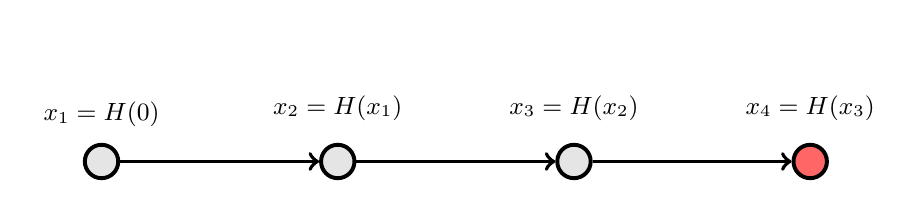
\begin{tikzpicture}
      [every node/.style={fill=gray!20,draw=black,circle,line width=0.5mm,inner sep=1.5mm}]
      \node[label={[yshift=-6mm]\small $x_1 = H(0)$}] (x1) at (0, 0) {};
      \node[label={[yshift=-6mm]\small $x_2 = H(x_1)$}] (x2) at (3, 0) {};
      \node[label={[yshift=-6mm]\small $x_3 = H(x_2)$}] (x3) at (6, 0) {};
      \node[fill=red!60,label={[yshift=-6mm]\small $x_4 = H(x_3)$}] (x4) at (9, 0) {};

      \draw[->,line width=0.5mm] (x1) -- (x2);
      \draw[->,line width=0.5mm] (x2) -- (x3);
      \draw[->,line width=0.5mm] (x3) -- (x4);
    \end{tikzpicture}
  \end{center}

  \pause
  Link nodes with hashes:
  \begin{itemize}[<+(1)->]
    \item 1\textsuperscript{st} node: $x_1 = H(0)$
    \item 2\textsuperscript{nd} node: $x_2 = H(x_1) = H\bigl(H(0)\bigr)$
    \item \dots
    \item i\textsuperscript{th} node: $x_i = H(x_{i-1}) = H\Bigl(H\bigl(\dots H(0)\dots\bigr)\Bigr)$
  \end{itemize}
\end{frame}

\begin{frame}{Hash-based structures}
  Hash trees (Merkle trees):
  \begin{itemize}[<+(1)->]
    \item Improvement to the linear nature of the chain
    \item Link elements in a tree structure (e.g. binary tree)
    \item Verify trail using intermediate nodes
    \item The root node must be monitored
  \end{itemize}
\end{frame}

\begin{frame}{(Binary) Merkle tree}
\only<1>{
  \colorlet{colorMerkleRoot}{gray!20}
  \colorlet{colorHashOneToFour}{gray!20}
  \colorlet{colorHashOneToTwo}{gray!20}
  \colorlet{colorHashThreeToFour}{gray!20}
  \colorlet{colorLeafThree}{yellow!60}
  \colorlet{colorLeafFour}{gray!20}
  \colorlet{colorHashFiveToEight}{gray!20}
}
\only<2->{
  \colorlet{colorLeafFour}{purple!60}
  \colorlet{colorHashThreeToFour}{teal!60}
  \colorlet{colorHashOneToTwo}{gray!20}
  \colorlet{colorHashOneToFour}{gray!20}
  \colorlet{colorHashFiveToEight}{gray!20}
  \colorlet{colorMerkleRoot}{gray!20}
}
\only<3->{
  \colorlet{colorHashOneToTwo}{purple!60}
  \colorlet{colorHashOneToFour}{teal!60}
  \colorlet{colorHashFiveToEight}{gray!20}
  \colorlet{colorMerkleRoot}{gray!20}
}
\only<4->{
  \colorlet{colorHashFiveToEight}{purple!60}
  \colorlet{colorMerkleRoot}{red!60}
}
  \vspace*{-3em}
  \begin{figure}
    \centering
    \begin{tikzpicture}
      [level distance=10mm,
      every node/.style={fill=colorMerkleRoot,draw=black,circle,line width=0.5mm,inner sep=1.5mm},
      edge from parent/.style={<-,draw},
      level 1/.style={sibling distance=40mm,line width=0.5mm,nodes={fill=gray!20}},
      level 2/.style={sibling distance=20mm,nodes={fill=gray!20}},
      level 3/.style={sibling distance=10mm,nodes={fill=gray!20}}]
      \node[label={[yshift=-13mm,visible on=<4->]north:\small $x_{\mathit{root}}=H(x_{1,4}||x_{5,8})$}] {}
        child {node[
          label={[visible on=<3->]left:{\small $x_{1,4}=H(x_{1,2}||x_{3, 4})$}},
          fill=colorHashOneToFour] {}
          child {node[label={left:\small $x_{1,2}=H(x_1||x_2)$},
                  fill=colorHashOneToTwo] {}
            child {node[label=south:{\small $x_1$}] {}}
            child {node[label=south:{\small $x_2$}] {}}
          }
          child {node[label={[xshift=-1mm,visible on=<2->]right:\small $x_{3,4}$},
                  fill=colorHashThreeToFour] {}
            child {node[label=south:{\small $x_3$},fill=yellow!60] {}}
            child {node[label=south:{\small $x_4$},fill=colorLeafFour] {}}
          }
        }
        child {node[label={[visible on=<4->]right:\small $x_{5,8}=H(x_{5,6}||x_{7,8})$},
                fill=colorHashFiveToEight] {}
          child {node {}
            child {node[label=south:{\small $x_5$}] {}}
            child {node[label=south:{\small $x_6$}] {}}
          }
          child {node {}
            child {node[label=south:{\small $x_7$}] {}}
            child {node[label=south:{\small $x_8$}] {}}
          }
        };
    \end{tikzpicture}
  \end{figure}
  \vspace*{-1em}
  \onslide<5->
  Knowing node $x_3$, we can verify the path to the root given only:
  \[
    H(x_4), H(x_{1,2}), H(x_{5,8}), H(x_{\mathit{root}})
  \]
\end{frame}

\begin{frame}{Widely witnessed evidence}
  \begin{figure}
    \centering
    \includegraphics[width=0.8\textwidth]{guardtime_root}
    \caption*{The Guardtime Merkle root published in a newspaper.}
  \end{figure}

  \pause
  {\scriptsize\url{https://x.com/Guardtime/status/1968214633048838434} most recent root}
\end{frame}

\begin{frame}{Message authentication codes (MAC)}
  \pause
  Authenticate and verify a message's integrity:
  \begin{itemize}[<+(1)->]
    \item authentication \emph{tag} requires a shared secret to compute
    \item any party with the secret can create valid MACs
    \item it should be infeasible to compute a valid MAC without the secret
    \item if the message is tampered with, the tag should not validate
  \end{itemize}
\end{frame}

\begin{frame}{MAC systems}
  A \emph{message authentication code} system is a triple of PPT algorithms:
  \begin{itemize}[<+(1)->]
    \item $\GEN$ is a \emph{key generation algorithm}: $k\gets\GEN()$
    \item $\MAC$ is a \emph{MAC generation algorithm}: $t\gets\MAC_k(m)$
    \item $\VERIF$ is a deterministic \emph{verification algorithm}: $b\gets\VERIF_k(m, t)$
  \end{itemize}

  \pause
  Notation and terms:
  \begin{itemize}[<+(1)->]
    \item $k$ -- shared secret \emph{authentication} key
    \item $b \in \{0, 1\}$ -- verification result
    \item $t$ is a valid \emph{tag} on $m$ under $k$ if $b = 1$
  \end{itemize}

  \pause
  The scheme is \emph{functional} if
  $\VERIF_k\bigl(m, \MAC_k(m)\bigr) = 1$.
\end{frame}

\begin{frame}{MAC scheme}
  \begin{center}
    \begin{tikzpicture}
      \node (alice) at (0,0)  {\includegraphics[height=80px]{alice}};
      \node (bob)   at (8, 0) {\includegraphics[height=80px]{bob}};
      \node (eve)   at (4, 0) {\includegraphics[height=80px]{eve}};

      \draw[<-, thick, visible on=<3->] (eve.east) -- node[above] {$\bigl(m, t\bigr)$} (bob.west);
      \draw[<-, thick, visible on=<4->] (alice.east) -- node[above] {$\bigl(m', t'\bigr)$} (eve.west);

      \node (gen)   at (4, 2) {$\GEN$};

      \node (ska) at (alice.north) [xshift=-7px,yshift=7px] {$k$};
      \node (skb) at (bob.north) [xshift=7px,yshift=7px] {$k$};

      \draw[<-,dashed,thick] (alice.north) |- (gen.west);
      \draw[->,dashed,thick] (gen.east) -| (bob.north);

      \node[anchor=west]  at (8.5, 0.25)  {$m\gets\MMM$};
      \node[anchor=west,visible on=<2->]  at (8.5, -0.25) {$t\gets\MAC_k(m)$};
      \node[anchor=north,visible on=<5->] at (alice.south) {$\VERIF_k(m, t)\iseq 1$};
    \end{tikzpicture}
  \end{center}

  \onslide<6->
  Mallory should not be able to \emph{forge} a valid tag.
\end{frame}

\begin{frame}{Security definitions}
  Attack scenarios
  \begin{itemize}[<+(1)->]
    \item \emph{Known-message attack} --
    Adversary sees some (message, tag) pairs.
    \item \emph{Chosen-message attack} --
    Adversary can adaptively request tags for messages of its choice.
  \end{itemize}

  \pause
  Attack types
  \begin{itemize}[<+(1)->]
    \item \emph{Universal forgery} --
    Create a valid tag for a given (any) message $m$.
    \item \emph{Existential forgery} --
    Create a valid tag for some message $m$.
  \end{itemize}

  \pause
  A MAC is \emph{unforgeable} if it is EUF-CMA secure
  \begin{itemize}[<+(1)->]
    \item Existential unforgeability under chosen-message attack
    \item Strong MAC: infeasible to create a different tag for a tagged message
  \end{itemize}
\end{frame}

\begin{frame}{MAC from CHF -- first attempt}
  Naive construction: SHA-256 with a secret key $k$
  \begin{itemize}[<+(1)->]
    \item Set the tag $t = \mathsf{SHA\text{-}256}(k||m)$ for some message $m$
    \item Recipient verifies $t$ by recomputing the hash
  \end{itemize}

  \vspace*{1em}

  \pause
  Insecure in most cases! {\scriptsize(Merkle-Damgård construction)}
  \begin{itemize}[<+(1)->]
    \item Insecure for variable-length messages: length extension attack
    \item More theoretically: generally not a pseudorandom function (PRF)
  \end{itemize}

  \vspace*{1em}

  \pause
  Hash functions are not random oracles!
\end{frame}

\begin{frame}{Length extension attack}
  Given $H(m_1)$ and $\lvert m_1\rvert$, an adversary can compute $H(m_1 || m_2)$ for some $m_2$.

  \vspace*{1em}

  \pause
  Vulnerable are:
  \begin{itemize}[<+(1)->]
    \item Hash functions based on Merkle-Damgård construction (iterative)
    \item E.g. MD5, SHA-1, non-truncated SHA-2
    \begin{itemize}
      \item SHA-256, SHA-512 but not\textsuperscript{*} SHA-384, SHA-512/256
      \item SHA-224 is truncated, but is weak against LE (32 bits of security)
      \item \textsuperscript{*}LE against SHA-384 and SHA-512/256 possible in theory, infeasible in practice 
    \end{itemize}
  \end{itemize}

  \pause
  {\scriptsize\url{https://github.com/iagox86/hash_extender} for a PoC}
\end{frame}

\begin{frame}{MAC from CHF -- second attempt}
  Naive construction: SHA-256 with a secret key $k$
  \begin{itemize}
    \item Set the tag $t = \mathsf{SHA\text{-}256}(m||k)$ for some message $m$
    \item Recipient verifies $t$ by recomputing the hash
  \end{itemize}

  \vspace*{1em}

  \pause
  Insecure if collisions are feasible! {\scriptsize(Merkle-Damgård construction)}
  \begin{itemize}[<+(1)->]
    \item $H(m) = H(m') \implies H(m||k) = H(m'||k)$
    \item Existential forgery if CR is broken
    \item Universal forgery if 2PIR is broken
  \end{itemize}
\end{frame}

\begin{frame}{HMAC}
  Hash-based message authentication code (HMAC)
  \begin{itemize}[<+(1)->]
    \item Used in and by KDFs
    \par
    \begin{itemize}
      \item HKDF constructed on top of HMAC
      \item PBKDF2 often used with HMAC, e.g. PBKDF2-HMAC-SHA256
    \end{itemize}
    \item Hash-function agnostic
    \par
    \begin{itemize}
      \item E.g. HMAC-SHA256, HMAC-SHA384, HMAC-SHA3-256
    \end{itemize}
    \item Security level depends on: key \& output length + security of hash
  \end{itemize}

  \vspace*{1em}

  \pause
  NB! Keyed hashing (HMAC) is not encryption
  \begin{itemize}
    \item HMAC is sometimes called \emph{keyed-hash} message authentication code
  \end{itemize}
\end{frame}

\begin{frame}{HMAC construction}
  \begin{columns}
    \begin{column}{0.4\textwidth}
      \begin{itemize}
        \item[] $H$ -- hash function
        \item[] $K$ -- HMAC key
        \vspace*{-1.25em}
        \item[] $K^+ \begin{cases}
          H(K) & \text{if\ } \lvert{}K\rvert > \text{block size}\\
          K & \text{otherwise}
        \end{cases}$
        \item[] $\mathit{ipad}$ -- inner padding (\texttt{0x36})
        \item[] $\mathit{opad}$ -- outer padding (\texttt{0x5c})
      \end{itemize}
    \end{column}
    \begin{column}{0.5\textwidth}
      \begin{figure}
    \centering
    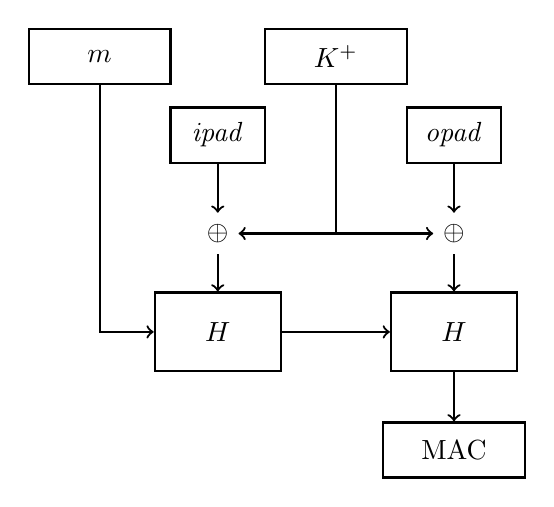
\begin{tikzpicture}[
      box/.style={draw, rectangle, minimum width=1.8cm, minimum height=0.7cm, align=center, thick},
      hashbox/.style={draw, rectangle, minimum width=1.6cm, minimum height=1.0cm, align=center, thick, font=\bfseries},
      arrow/.style={->, thick},
      xor/.style={minimum size=0.5cm, thick, inner sep=0pt}
    ]
      \node[box] (msg) at (0, 0) {$m$};
      \node[box] (key) at (3, 0) {$K^+$};

      \node[box, minimum width=1.2cm] (ipad) at (1.5, -1) {$\mathit{ipad}$};
      \node[box, minimum width=1.2cm] (opad) at (4.5, -1) {$\mathit{opad}$};

      \node[xor] (xor1) at (1.5, -2.25) {$\oplus$};
      \node[xor] (xor2) at (4.5, -2.25) {$\oplus$};

      \node[hashbox] (hash1) at (1.5, -3.5) {$H$};
      \node[hashbox] (hash2) at (4.5, -3.5) {$H$};

      %\node (hprime) at (3.2, -3.8) {$H' \leftarrow \mathit{HASH}(\overline{K_1}||M)$};
      %\node (hdprime) at (5, -5.2) {$H'' \leftarrow \mathit{HASH}(\overline{K_2}||H')$};
      \node[box, draw, thick] (mac) at (4.5, -5) {MAC};

      \draw[arrow] (msg) -- (0, -3.5) -- (hash1.west);

      \draw[arrow] (key) -- (3, -2.25) -- (xor1.east);
      \draw[arrow] (key) -- (3, -2.25) -- (xor2.west);
      \draw[arrow] (ipad) -- (xor1);
      \draw[arrow] (opad) -- (xor2);

      \draw[arrow] (xor1) -- (hash1);
      \draw[arrow] (xor2) -- (hash2);

      \draw[arrow] (hash1.east) -- (hash2.west);
      \draw[arrow] (hash2.south) -- (mac.north);
    \end{tikzpicture}
  \end{figure}
    \end{column}
  \end{columns}
  \pause
  \scriptsize{You do not need to remember this construction}
\end{frame}

\begin{frame}{MAC from CBC}
  \pause
  \begin{figure}
    \centering
    \begin{tikzpicture}
      \foreach \x in {1, 2, 3} {
        \node (f\x) at ($\x*(2.5cm,0)$) [minimum size=1.25cm,fill=gray!20,draw] {$\ENC$};
        \node (p\x) [above of=f\x, node distance=1.5cm, circle, draw] {};
        \node (m\x) [above of=p\x, node distance=1cm] {$m_\x$};
        \node (k\x) [left of=f\x, node distance=1.5cm] {$k$};
        \node (c\x) [below of=f\x, node distance=0.77cm] {};

        \draw[-] (p\x.east) -- (p\x.west);

        \draw[-latex] (m\x) -- (f\x);
        \draw[-latex] (k\x) -- (f\x);
        \draw[-] (f\x) -- (c\x.center);
      }

      \node (iv) [left of=p1, node distance=2cm] {$0^b$};
      \draw[-latex] (iv) -- (p1);

      \node (t) [below of=f3, node distance=1.5cm] {$t$};
      \draw[-latex] (f3) -- (t);

      \foreach \x in {1, 2} {
          \pgfmathtruncatemacro{\next}{\x+1}
          \draw[-latex] (c\x.center) -| ($(p\next.west) + (-1.53cm, 0)$) -- (p\next.west);
      }
    \end{tikzpicture}
  \end{figure}

  \pause
  \begin{itemize}
    \item The IV is fixed (typically $0^b$ for block-length $b$)
    \item The MAC tag is the last ciphertext block
    \pause
    \item Insecure for variable-length messages + other pitfalls
  \end{itemize}
\end{frame}

\begin{frame}{Construction takeaway}
  Do not build your own MACs!
  \begin{itemize}[<+(1)->]
    \item Use special-purpose MAC algorithms
    \item Ensure the key-length is sufficient
    \item Use parameters suggested by reputable sources
    \item Not all MACs are hash-based, e.g. CMAC, GMAC
  \end{itemize}
\end{frame}

\begin{frame}{What to use}
  First, check what the documentation/standard recommends for your use case.
  \begin{itemize}
    \item AEADs typically specify encryption + MAC pair
    \item E.g. Poly1305 for ChaCha20
  \end{itemize}

  \vspace*{1em}

  \pause
  In a standalone setting (no confidentiality), use
  \begin{itemize}[<+(1)->]
    \item HMAC: hash-based message authentication code
    \begin{itemize}
      \item Commonly used with SHA-2 family hashes
      \item Usable with any CHF
      \item \href{https://datatracker.ietf.org/doc/html/rfc2104}{RFC 2104}, \href{https://csrc.nist.gov/pubs/fips/198-1/final}{FIPS 198-1} (migration in progress to \href{https://csrc.nist.gov/pubs/sp/800/224/ipd}{SP 800-224})
    \end{itemize}
    \item KMAC: Keccak MAC
    \begin{itemize}
      \item \href{https://csrc.nist.gov/pubs/sp/800/185/final}{NIST SP 800-185} (planned \href{https://csrc.nist.gov/news/2025/decision-to-update-fips-202-and-revise-sp-800-185}{\textit{revision}})
    \end{itemize}
  \end{itemize}
\end{frame}

\begin{frame}{What to use}
  For authenticated encryption, use standard AEAD schemes:
  \begin{itemize}[<+(1)->]
    \item AES-GCM {\scriptsize(or AES-GCM-SIV for nonce-misuse resistance)}
    \item (X)ChaCha20-Poly1305
  \end{itemize}

  \vspace*{1em}

  \pause
  If composing encryption and MAC yourself:
  \begin{itemize}[<+(1)->]
    \item Encrypt-then-MAC (EtM)
    \item MAC the ciphertext \emph{and} the nonce/IV
    \item Use separate keys for encryption and MAC
    \item AES-CTR + HMAC-SHA2XX in EtM mode
  \end{itemize}

  \vspace*{1em}

  \pause
  Never reuse nonces under the same key!
\end{frame}

\begin{frame}{Recap}
  MACs provide data authenticity and integrity
  \begin{itemize}[<+(1)->]
    \item Use established schemes (e.g. HMAC); do not design your own
    \item Messages need not be confidential
    \item Tags may leak information about the message
  \end{itemize}

  \vspace*{1em}

  \pause
  Symmetric encryption typically needs to be authenticated
  \begin{itemize}[<+(1)->]
    \item Prefer established AEAD constructions
    \item Encrypt-then-MAC (EtM): authenticate the ciphertext and nonce/IV
    \item Use separate keys for encryption and MAC
  \end{itemize}
\end{frame}

\end{document}
